\documentclass[11pt]{article}
\usepackage[utf8]{inputenc}
\usepackage[T1]{fontenc}
\usepackage{amsmath,amssymb}
\usepackage{booktabs}
\usepackage{graphicx}
\usepackage{hyperref}
\usepackage{xcolor}
\usepackage{multirow}
\usepackage[margin=1in]{geometry}
\usepackage{natbib}
\usepackage{caption}
\usepackage{subcaption}
\usepackage{tikz}
\usetikzlibrary{arrows.meta,positioning,fit,backgrounds,calc}

\title{MKOS: A Biomimetic Architecture for Knowledge Base Quality Management}

\author{
  Michael Munz\\
  Independent Researcher\\
  Germany\\
  \texttt{[email on request]}
}

\date{}

\begin{document}
\maketitle

\begin{abstract}
Internal and proprietary knowledge bases---powering enterprise RAG systems, decision support, and organizational memory---accumulate quality issues over time: hallucinations, staleness, bias, and contradictions that degrade downstream reliability. Unlike public knowledge, these issues cannot be caught by an LLM's parametric knowledge alone, as the model has no training data for proprietary content. We present MKOS (Mycelial Knowledge Operating System), a biomimetic architecture that applies biological immune system principles to automated knowledge quality management. MKOS employs a two-phase detection pipeline: (1) an innate classifier that gates healthy content with a single LLM call, and (2) specialized adaptive detectors that perform retrieval-augmented deep analysis for flagged threats. Additional biomimicry subsystems---stigmergic coordination, quorum sensing, and homeostatic self-regulation---enable cross-component signaling and autonomous parameter tuning.

We introduce \textbf{KQAB} (Knowledge Quality Assurance Benchmark), a 4-task evaluation suite covering threat detection, contradiction discovery, temporal decay, and evidence grounding, with both author-constructed synthetic (584 items, single annotator) and public dataset variants adapted from MNLI and FEVER (923 items total). On the author-constructed T1 benchmark, MKOS achieves Macro-F1=0.975 on 5-class threat detection, significantly outperforming both LLM few-shot (F1=0.842) and chain-of-thought (F1=0.816) baselines using the same underlying model (McNemar $p{<}0.003$, permutation test $p{<}0.003$)---with the advantage concentrated on internal-KB-like content where the LLM lacks prior knowledge. An ablation study across 10 configurations confirms that the multi-detector ensemble is essential (innate-only F1=0.139) and that all four specialized detectors contribute measurably. A proof-of-concept RAG evaluation (30 items) shows that MKOS filtering raises downstream answer correctness from 0.850 to 1.000. We release MKOS as open-source software with reproducible benchmarks. \emph{Caveat:} These results rest on a small, single-annotator dataset without inter-annotator agreement measurement; independent validation is needed before definitive claims can be made.
\end{abstract}

\section{Introduction}
\label{sec:intro}

Knowledge bases (KBs) are foundational infrastructure for retrieval-augmented generation (RAG), enterprise search, and decision-support systems. As KBs grow, they inevitably accumulate quality issues: factual errors introduced during ingestion (hallucinations), information that becomes outdated as technology evolves (staleness), single-perspective presentations that omit alternatives (bias), and claims that contradict other KB entries or established facts (contradictions).

For \emph{internal} and \emph{proprietary} KBs---company wikis, product documentation, organizational policies---these issues are particularly insidious. An LLM has no parametric knowledge of proprietary content, so naive approaches that rely on the model's training data (e.g., few-shot classification) cannot verify internal claims against ground truth. Quality management requires \emph{retrieval-augmented} verification against the KB itself.

Existing approaches to KB quality management are predominantly manual---expert review, periodic audits, user-reported errors---and scale poorly with KB size. Automated fact-checking systems \citep{thorne2018fever, guo2022survey} focus on verifying individual claims against external corpora but do not address the full spectrum of quality issues within a managed knowledge base. Hallucination detection benchmarks \citep{li2023halueval, lin2022truthfulqa} evaluate LLM output quality rather than the quality of \emph{stored knowledge}.

We propose MKOS, a system inspired by biological immune systems that treats knowledge quality issues as \emph{pathogens} requiring detection, classification, and remediation. Our key contributions are:

\begin{enumerate}
    \item \textbf{A two-phase immune architecture} that combines fast innate classification (1 LLM call) with deep adaptive analysis by specialized detectors, achieving F1=0.975 on 5-class threat detection.
    \item \textbf{KQAB}, a benchmark suite for evaluating KB quality systems across four tasks, including two author-constructed tasks (threat detection, temporal decay) and two adaptations of established NLI and fact-verification datasets (MNLI \citep{williams2018broad}, FEVER \citep{thorne2018fever}).
    \item \textbf{Biomimicry subsystems}---stigmergy, quorum sensing, and homeostasis---that enable autonomous cross-component coordination and self-regulation.
    \item \textbf{End-to-end RAG evaluation} showing that MKOS filtering raises downstream answer correctness by 15 percentage points, and \textbf{knowledge graph contradiction detection} as a complementary structural analysis modality.
    \item \textbf{An ablation study} demonstrating that both the two-phase architecture and the multi-detector ensemble are essential for strong performance.
\end{enumerate}

\section{Related Work}
\label{sec:related}

\paragraph{Knowledge Base Quality.} KB quality management has been studied in the context of knowledge graphs \citep{paulheim2017knowledge, zaveri2016quality}, where completeness, consistency, and timeliness are primary concerns. These approaches typically rely on structural constraints (ontology validation, type checking) rather than semantic analysis. MKOS targets \emph{unstructured} knowledge bases where content is stored as natural language text.

\paragraph{Automated Fact Checking.} Systems like FEVER \citep{thorne2018fever} and fact-verification pipelines \citep{guo2022survey} retrieve evidence and classify claims as supported, refuted, or unverifiable. MKOS extends this paradigm by classifying quality issues into four threat types and operating on \emph{internal} KB content rather than external claims.

\paragraph{Hallucination Detection.} Recent work on LLM hallucination detection \citep{li2023halueval, manakul2023selfcheckgpt} focuses on identifying unsupported claims in generated text. MKOS applies similar principles to stored knowledge, using retrieval-augmented verification against the KB itself.

\paragraph{Biomimicry in Computing.} Artificial immune systems (AIS) have been applied to network intrusion detection \citep{dasgupta2011advances}, anomaly detection, and optimization. Stigmergy-based coordination has been explored in swarm robotics and distributed systems \citep{theraulaz1999brief}. MKOS adapts these biological metaphors specifically to knowledge quality management.

\section{Architecture}
\label{sec:arch}

MKOS consists of three core subsystems: the Knowledge Immune System (\S\ref{sec:kis}), biomimicry coordination (\S\ref{sec:biomimicry}), and the knowledge lifecycle pipeline (\S\ref{sec:lifecycle}).

\subsection{Knowledge Immune System (KIS)}
\label{sec:kis}

KIS employs a two-phase architecture inspired by biological immunity (Figure~\ref{fig:pipeline}):

\begin{figure}[h]
\centering
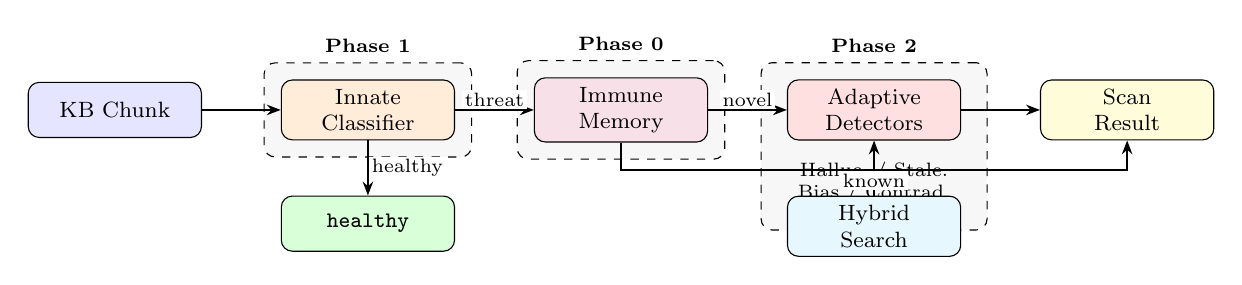
\begin{tikzpicture}[
    node distance=0.6cm and 0.8cm,
    box/.style={draw, rounded corners, minimum width=2.2cm, minimum height=0.7cm, align=center, font=\footnotesize},
    phase/.style={draw, dashed, rounded corners=4pt, inner sep=6pt, fill=black!3},
    arr/.style={-{Stealth[length=5pt]}, thick},
    lbl/.style={font=\scriptsize, fill=white, inner sep=1pt},
]
% Input
\node[box, fill=blue!10] (input) {KB Chunk};

% Phase 1
\node[box, fill=orange!15, right=1.0cm of input] (innate) {Innate\\Classifier};

% Gate decision
\node[box, fill=green!15, below=0.7cm of innate] (healthy) {\texttt{healthy}};

% Phase 0
\node[box, fill=purple!12, right=1.0cm of innate] (memory) {Immune\\Memory};

% Phase 2 detectors
\node[box, fill=red!12, right=1.0cm of memory] (detectors) {Adaptive\\Detectors};

% Detector details below
\node[font=\scriptsize, below=0.15cm of detectors, text width=2.2cm, align=center] (dlist) {Halluc.\ / Stale.\\Bias / Contrad.};

% Output
\node[box, fill=yellow!15, right=1.0cm of detectors] (output) {Scan\\Result};

% Hybrid search
\node[box, fill=cyan!10, below=0.7cm of detectors] (search) {Hybrid\\Search};

% Arrows
\draw[arr] (input) -- (innate);
\draw[arr] (innate) -- node[lbl, above] {threat} (memory);
\draw[arr] (innate) -- node[lbl, right] {healthy} (healthy);
\draw[arr] (memory) -- node[lbl, above] {novel} (detectors);
\draw[arr] (detectors) -- (output);
\draw[arr] (search) -- (detectors);

% Memory shortcut
\draw[arr] (memory.south) -- ++(0,-0.35) -| node[lbl, near start, below] {known} (output.south);

% Phase labels
\begin{scope}[on background layer]
\node[phase, fit=(innate), label={[font=\scriptsize\bfseries]above:Phase 1}] {};
\node[phase, fit=(memory), label={[font=\scriptsize\bfseries]above:Phase 0}] {};
\node[phase, fit=(detectors)(dlist), label={[font=\scriptsize\bfseries]above:Phase 2}] {};
\end{scope}
\end{tikzpicture}
\caption{Knowledge Immune System pipeline. Phase~1 (innate classifier) gates healthy content with a single LLM call. Flagged threats check immune memory (Phase~0) for known patterns; novel threats proceed to specialized adaptive detectors (Phase~2) that use hybrid search for evidence retrieval.}
\label{fig:pipeline}
\end{figure}

\paragraph{Phase 1: Innate Response.} A single LLM call classifies content into one of five categories: \texttt{healthy}, \texttt{hallucination}, \texttt{staleness}, \texttt{bias}, or \texttt{contradiction}. The innate classifier uses a structured few-shot prompt with decision rules and examples. If the classifier returns \texttt{healthy}, no further analysis occurs---this \emph{gating} mechanism reduces LLM calls by approximately 50\%.

\paragraph{Phase 0: Immune Memory.} Before adaptive analysis, the system checks for known pathogen patterns in immune memory. Patterns are stored with multi-keyword signatures (requiring 2+ keyword matches, with stop-word filtering to prevent false matches). Matched patterns bypass adaptive analysis, enabling sub-millisecond re-detection.

\paragraph{Phase 2: Adaptive Response.} For content flagged as a threat, a specialized detector performs deep analysis:

\begin{itemize}
    \item \textbf{HallucinationDetector}: Retrieves related KB chunks via hybrid search (FTS5 + vector, RRF fusion) and prompts the LLM to compare claims against retrieved evidence.
    \item \textbf{StalenessDetector}: Identifies outdated version references, deprecated technologies, and date-specific claims.
    \item \textbf{BiasDetector}: Detects single-perspective presentation, absolutist language, and missing counterarguments.
    \item \textbf{ContradictionDetector}: Two strategies---FTS-context comparison against related chunks, plus established-facts fallback for isolated contradictions.
\end{itemize}

\paragraph{Innate-Label Priority.} For the ambiguous boundary between bias and contradiction (both involve ``opposing'' language), the system runs both detectors but \emph{prefers the detector matching the innate label}. If the innate-labeled detector finds threats, the other detector's results are discarded. This optimization raised contradiction F1 from 0.064 to 0.933 by eliminating cross-classification.

\subsection{Biomimicry Coordination}
\label{sec:biomimicry}

Three biological coordination mechanisms enable autonomous system behavior. Table~\ref{tab:biomimicry} maps each biological metaphor to its concrete software implementation.

\begin{table}[h]
\centering
\caption{Biomimicry concepts and their software implementations}
\label{tab:biomimicry}
\begin{tabular}{lll}
\toprule
\textbf{Biological Term} & \textbf{Software Implementation} & \textbf{Mechanism} \\
\midrule
Innate immunity & Few-shot LLM classifier & Fast gate (1 call) \\
Adaptive immunity & Specialized detector ensemble & Deep analysis \\
Immune memory & Pattern store + keyword match & Sub-ms re-detection \\
Stigmergy & Event-driven signal table & Async DB flags w/ decay \\
Quorum sensing & Threshold-based aggregation & Grouped metric triggers \\
Homeostasis & PID-like control loop & Setpoint-driven tuning \\
Composting & Entropy-based archival & $E(t) = 1-e^{-\lambda\Delta t}$ \\
Fermentation & Cross-ref staging pipeline & Confidence scoring \\
\bottomrule
\end{tabular}
\end{table}

\paragraph{Stigmergy.} Subsystems communicate indirectly through pheromone signals stored in a shared signal table. Signals carry a type (e.g., \texttt{THREAT\_DETECTED}), domain, intensity, and source. Repeated signals in the same domain \emph{reinforce}, while all signals \emph{decay} exponentially (72-hour half-life). The fermentation subsystem reads domain threat levels to apply confidence penalties to incoming content in high-threat domains.

\paragraph{Quorum Sensing.} When the number of unresolved threats in a domain exceeds a configurable threshold (e.g., 3 for hallucination), collective actions are triggered: domain quarantine, cascade composting, batch rescan, or raised scrutiny. This prevents localized quality issues from spreading.

\paragraph{Homeostasis.} The system continuously measures vital signs---threat rate, false-positive rate, average entropy, composting throughput, fermentation rejection rate---and compares them against setpoints. When metrics drift outside healthy ranges, the regulator recommends parameter adjustments (e.g., increasing confidence thresholds in high-threat domains).

\subsection{Knowledge Lifecycle}
\label{sec:lifecycle}

Two additional subsystems manage knowledge lifecycle:

\paragraph{Composting.} An entropy-based decay model, $E(t) = 1 - \exp(-\lambda \cdot \Delta t)$, scores knowledge freshness. High-entropy chunks are decomposed into reusable \emph{nutrients}---principles, patterns, error patterns, meta-insights---stored with FTS5 indexing for future enrichment.

\paragraph{Fermentation.} New content enters a staging chamber, is cross-referenced against existing knowledge via hybrid search, and receives a confidence score based on supporting references and detected contradictions. Content is promoted or rejected based on configurable thresholds.

\section{KQAB: Knowledge Quality Assurance Benchmark}
\label{sec:kqab}

Existing benchmarks evaluate either LLM output quality (TruthfulQA, HaluEval) or individual claim verification (FEVER). None evaluate the quality of \emph{stored knowledge} in a managed KB. We introduce KQAB, a 4-task benchmark with three dataset variants.

\subsection{Tasks}

\begin{itemize}
    \item \textbf{T1: Threat Detection} (5-class). Classify KB chunks as \texttt{healthy}, \texttt{hallucination}, \texttt{staleness}, \texttt{bias}, or \texttt{contradiction}. Primary metric: Macro-F1.
    \item \textbf{T2: Contradiction Discovery} (3-class). Given a chunk pair, classify as \texttt{contradicts}, \texttt{consistent}, or \texttt{unrelated}. Tests inter-chunk consistency analysis.
    \item \textbf{T3: Temporal Decay Detection} (3-class). Classify KB content as \texttt{current}, \texttt{outdated}, or \texttt{deprecated}. Tests temporal awareness.
    \item \textbf{T4: Evidence Grounding} (3-class). Given a claim and KB context, classify as \texttt{supported}, \texttt{unsupported}, or \texttt{partial}. Tests retrieval-based verification.
\end{itemize}

\subsection{Dataset Variants}

\paragraph{KQAB-Synth} (584 items). Author-constructed items covering software engineering, data science, and general technical knowledge, designed to simulate quality issues in internal knowledge bases where the LLM has no training data. T1: 321 items with balanced threat-type representation. T3 expanded to 200 items covering both SE and general knowledge domains. All synthetic items and generation code are released for community review and extension.

\paragraph{KQAB-Public} (923 items). Adaptations of established NLP datasets for KB-specific evaluation:
\begin{itemize}
    \item T2: 201 items from Multi-Genre NLI \citep{williams2018broad}. Label mapping: entailment$\to$\texttt{consistent}, contradiction$\to$\texttt{contradicts}, neutral$\to$\texttt{unrelated}. Balanced at 67 items per class.
    \item T4: 201 items from FEVER \citep{thorne2018fever}. Label mapping: SUPPORTS$\to$\texttt{supported}, REFUTES$\to$\texttt{unsupported}, NOT\_ENOUGH\_INFO$\to$\texttt{partial}. Balanced at 67 items per class.
\end{itemize}

T1 and T3 use synthetic items in both variants, as no public dataset exists for KB-specific threat detection or temporal decay classification.

\section{Experiments}
\label{sec:experiments}

\subsection{Setup}

All experiments use Claude Sonnet 4 (Anthropic) as the underlying LLM unless otherwise noted. A SQLite-backed LLM response cache ensures deterministic results across runs ($\sigma=0.0$). Total benchmark cost: \$5.15 across all experiments.

\paragraph{Systems Compared.}
\begin{itemize}
    \item \textbf{MKOS AIS}: Full two-phase immune system with all four adaptive detectors.
    \item \textbf{LLM Few-Shot}: Same LLM with a single few-shot classification prompt. No retrieval, no memory, no specialized detectors.
    \item \textbf{Regex Heuristic}: Keyword-matching baseline.
\end{itemize}

\subsection{T1: Threat Detection Results}

Table~\ref{tab:t1} shows results on the 321-item synthetic dataset.

\begin{table}[h]
\centering
\caption{T1 Threat Detection (n=321, Macro-F1)}
\label{tab:t1}
\begin{tabular}{lcccc}
\toprule
\textbf{System} & \textbf{Precision} & \textbf{Recall} & \textbf{Macro-F1} \\
\midrule
Regex Heuristic & 1.000 & 0.060 & 0.113 \\
LLM Few-Shot & 0.986 & 0.953 & 0.842 \\
LLM Chain-of-Thought & 0.955 & 0.860 & 0.816 \\
\textbf{MKOS AIS} & \textbf{0.987} & \textbf{0.987} & \textbf{0.975} \\
\bottomrule
\end{tabular}
\end{table}

\paragraph{Per-Class Analysis.} Table~\ref{tab:perclass} reveals that MKOS outperforms both Few-Shot and Chain-of-Thought on \emph{every} threat class. CoT underperforms Few-Shot overall, with the largest MKOS advantages over CoT on bias (+26.9pp) and contradiction (+29.0pp).

\begin{table}[h]
\centering
\caption{Per-class F1 on T1 (n=321)}
\label{tab:perclass}
\begin{tabular}{lcccc}
\toprule
\textbf{Class} & \textbf{AIS F1} & \textbf{CoT F1} & \textbf{Few-Shot F1} & \textbf{$\Delta$ AIS--CoT} \\
\midrule
Hallucination & 0.980 & 0.905 & 0.938 & +7.5pp \\
Staleness & 0.987 & 0.873 & 0.919 & +11.4pp \\
Bias & 0.983 & 0.714 & 0.735 & +26.9pp \\
Contradiction & 0.933 & 0.643 & 0.654 & +29.0pp \\
Healthy & 0.988 & 0.943 & 0.966 & +4.5pp \\
\bottomrule
\end{tabular}
\end{table}

\subsection{KQAB Multi-Task Results}

\begin{table}[h]
\centering
\caption{KQAB results across all tasks (Macro-F1)}
\label{tab:kqab}
\begin{tabular}{llccc}
\toprule
\textbf{Variant} & \textbf{Task} & \textbf{MKOS} & \textbf{Few-Shot} & \textbf{n} \\
\midrule
\multirow{4}{*}{Synth}
& T1: Threat Detection & \textbf{0.975} & 0.842 & 321 \\
& T2: Contradiction & \textbf{1.000} & \textbf{1.000} & 35 \\
& T3: Temporal Decay & \textbf{0.872} & 0.860 & 200 \\
& T4: Evidence Grounding & \textbf{0.898} & 0.867 & 28 \\
\midrule
\multirow{3}{*}{Public}
& T2: Contradiction (MNLI) & 0.612 & 0.613 & 201 \\
& T3: Temporal Decay & \textbf{0.905} & 0.894 & 200 \\
& T4: Grounding (FEVER) & \textbf{0.593} & 0.586 & 201 \\
\bottomrule
\end{tabular}
\end{table}

On KQAB-Public, MKOS consistently matches or outperforms Few-Shot on specialized tasks (T3, T4). The T2 drop from 1.000 to 0.612 on MNLI reflects the greater nuance of real NLI data---both systems struggle equally with the neutral/unrelated class (F1$\approx$0.2). We note that T2-Synth (n=35) and T4-Synth (n=28) are too small for reliable conclusions; the perfect F1=1.000 on T2-Synth likely reflects dataset simplicity rather than system capability. The public-dataset variants (n=201 each) provide the more meaningful comparison for these tasks.

\subsection{Ablation Study}

We systematically evaluate component contributions by enabling/disabling detectors (Table~\ref{tab:ablation}).

\begin{table}[h]
\centering
\caption{Ablation study on T1 (n=321, 10 configurations)}
\label{tab:ablation}
\begin{tabular}{lcc}
\toprule
\textbf{Configuration} & \textbf{Macro-F1} & \textbf{$\Delta$ vs Full} \\
\midrule
Full AIS (4 detectors) & \textbf{0.975} & --- \\
Innate only (no adaptive) & 0.139 & $-$0.836 \\
\midrule
Without hallucination & 0.752 & $-$0.223 \\
Without staleness & 0.757 & $-$0.218 \\
Without contradiction & 0.722 & $-$0.253 \\
Without bias & 0.745 & $-$0.230 \\
\midrule
Only hallucination & 0.352 & $-$0.623 \\
Only staleness & 0.349 & $-$0.626 \\
Only contradiction & 0.314 & $-$0.661 \\
Only bias & 0.288 & $-$0.687 \\
\bottomrule
\end{tabular}
\end{table}

Key findings: (1) The adaptive phase is critical---innate-only achieves F1=0.139, confirming it serves as a gate, not a classifier. (2) All four detectors contribute approximately equally ($\Delta$=0.218--0.253 for leave-one-out). (3) No single detector is sufficient (F1=0.288--0.352 for single-detector configs).

\subsection{Multi-Model Evaluation}

To test model sensitivity, we evaluated with GPT-4o (Table~\ref{tab:multimodel}).

\begin{table}[h]
\centering
\caption{Multi-model evaluation on T1 (n=321)}
\label{tab:multimodel}
\begin{tabular}{lcc}
\toprule
\textbf{System} & \textbf{Claude Sonnet 4} & \textbf{GPT-4o} \\
\midrule
AIS & \textbf{0.975} & 0.869 \\
Few-Shot & 0.842 & \textbf{0.977} \\
\bottomrule
\end{tabular}
\end{table}

The architecture is model-sensitive: Claude AIS (0.975) significantly outperforms GPT-4o AIS (0.869), while raw few-shot performance is comparable across models. This indicates that detector prompts require model-specific tuning.

\subsection{Biomimicry Validation}

Functional testing of all three biomimicry subsystems achieves 100\% pass rate (8/8 tests): stigmergy signal propagation and decay, quorum sensing activation above threshold, and homeostatic parameter diagnosis (see supplementary material).

\subsection{Real-World Dataset}

A 225-item dataset constructed from Wikipedia article summaries (43 technical topics) with programmatic perturbations shows that Few-Shot (F1=0.976) outperforms AIS (F1=0.963) on \emph{public knowledge}. This is expected: programmatic perturbations to well-known facts are detectable by the LLM's parametric knowledge alone. MKOS's retrieval-based architecture adds the most value on \emph{internal} knowledge bases where the LLM has no prior training data.

\subsection{Zero-Shot Enterprise Domain}
\label{sec:zero-shot}

To test MKOS on truly proprietary content, we constructed a 179-item knowledge base for a \emph{fictional} company (``Nexara Technologies'') with five invented products. The LLM has zero training data for this content. We evaluate five configurations to disentangle the effects of the innate gate and domain calibration (Table~\ref{tab:zeroshot}).

To prevent data leakage, we use a stratified holdout split: 48 items for calibration (3 few-shot examples per class), 131 items for evaluation. Calibration and evaluation sets are strictly disjoint.

\begin{table}[h]
\centering
\caption{Zero-Shot Enterprise Domain (n\textsubscript{eval}=131, n\textsubscript{cal}=48, stratified holdout). Gate bypass = innate gate disabled, all chunks reach adaptive detectors. Auto-cal.\ = domain-specific few-shot examples from held-out calibration set.}
\label{tab:zeroshot}
\begin{tabular}{lccccc}
\toprule
\textbf{System} & \textbf{Macro-F1} & \textbf{Halluc.} & \textbf{Stale.} & \textbf{Bias} & \textbf{Contrad.} \\
\midrule
MKOS (uncalibrated) & 0.339 & 0.444 & 0.087 & 0.667 & 0.138 \\
MKOS + gate bypass & 0.264 & 0.349 & 0.087 & 0.667 & 0.216 \\
\textbf{MKOS + auto-cal.} & \textbf{0.852} & \textbf{0.955} & \textbf{0.829} & 0.977 & \textbf{0.667} \\
MKOS + auto-cal.\ + gate bypass & 0.580 & 0.500 & 0.829 & \textbf{0.977} & 0.596 \\
Few-Shot & 0.566 & 0.620 & 0.412 & \textbf{1.000} & 0.167 \\
\bottomrule
\end{tabular}
\end{table}

\paragraph{Auto-Calibration as Primary Fix.} Automatic calibration---sampling 48 chunks from the target KB (stratified, disjoint from the evaluation set) and injecting 3 per class as domain-specific few-shot examples into the innate classifier---transforms zero-shot performance from F1=0.339 to \textbf{0.852} (+51.3pp), exceeding Few-Shot by +28.6pp on held-out data. The calibrated innate gate correctly routes threats to adaptive detectors: hallucination F1 rises from 0.444 to 0.955, staleness from 0.087 to 0.829, and contradiction from 0.138 to 0.667. This confirms that the innate gate's domain miscalibration was the primary bottleneck: once the gate receives domain-representative examples, the full two-phase architecture recovers its advantage even on completely novel content.

\paragraph{Gate Bypass Hurts, Not Helps.} Counter to our initial hypothesis, bypassing the innate gate \emph{degrades} performance in both the uncalibrated (0.339$\to$0.264, $-$7.5pp) and calibrated (0.852$\to$0.580, $-$27.2pp) settings. The mechanism is clear: without the gate, all chunks are forwarded to all four adaptive detectors, and healthy chunks are frequently misclassified as threats (healthy F1=0.000 in both bypass conditions). The innate gate, even when imperfectly calibrated, provides essential \emph{specificity}---it suppresses false positives that overwhelm the adaptive phase. This is analogous to the immunological principle that an innate response must have reasonable specificity before triggering the more sensitive (but less specific) adaptive response.

\paragraph{Calibration Efficiency.} How many examples per class are needed? We vary $k \in \{1, 3, 5, 10\}$ with stratified holdout splits (Table~\ref{tab:calcurve}).

\begin{table}[h]
\centering
\caption{Calibration curve: F1 on held-out Nexara data as a function of examples per class ($k$)}
\label{tab:calcurve}
\begin{tabular}{cccc}
\toprule
\textbf{$k$} & \textbf{$n_\text{cal}$} & \textbf{$n_\text{eval}$} & \textbf{Macro-F1 [95\% CI]} \\
\midrule
1 & 5 & 174 & 0.845 [0.850, 0.938] \\
\textbf{3} & \textbf{15} & \textbf{164} & \textbf{0.869 [0.872, 0.952]} \\
5 & 25 & 154 & 0.858 [0.859, 0.948] \\
10 & 50 & 129 & 0.839 [0.832, 0.941] \\
\bottomrule
\end{tabular}
\end{table}

Calibration saturates almost immediately: even $k$=1 (5 items total) achieves F1=0.845, and all confidence intervals overlap substantially. The peak at $k$=3 (F1=0.869) reflects the balance between calibration quality and evaluation set size. This means that a practical deployment requires labeling as few as 5--15 domain items---no fine-tuning, no retraining, just prompt augmentation---to recover near-full performance on completely novel content.

\subsection{End-to-End RAG Impact}
\label{sec:rag}

To measure MKOS's downstream utility, we evaluate answer quality in a retrieval-augmented generation (RAG) pipeline under three conditions: (1)~\emph{Degraded}---the KB contains both healthy and threat chunks without filtering; (2)~\emph{Filtered}---MKOS scans and removes detected threats before RAG retrieval; (3)~\emph{Clean}---an oracle KB containing only healthy chunks. We construct a 30-item KB across 10 technical domains (Python, Docker, SQL, Kubernetes, REST, Git, ML, Security, Caching, Testing), each with 2 healthy chunks and 1 threat. An LLM-as-judge evaluates correctness (factual accuracy) and faithfulness (grounding in retrieved context) for 10 domain-specific questions.

\begin{table}[h]
\centering
\caption{End-to-end RAG quality under three KB conditions}
\label{tab:rag}
\begin{tabular}{lccc}
\toprule
\textbf{Metric} & \textbf{Degraded} & \textbf{MKOS-Filtered} & \textbf{Clean Oracle} \\
\midrule
Correctness & 0.850 & \textbf{1.000} & 1.000 \\
Faithfulness & 0.880 & \textbf{1.000} & 1.000 \\
Threat usage rate & 100\% & 0\% & 0\% \\
\bottomrule
\end{tabular}
\end{table}

MKOS filtering eliminates all 10/10 threat chunks (detection rate=100\%), raising correctness from 0.850 to 1.000 (+15pp) and matching the clean oracle condition. This demonstrates that upstream quality filtering has a measurable, practical impact on downstream answer reliability.

\subsection{Knowledge Graph Contradiction Detection}
\label{sec:kg}

While the per-chunk immune system classifies individual items in isolation, some contradictions are only detectable through \emph{structural} analysis across chunks. We build an entity-relation knowledge graph over the full T1 dataset (321 chunks) by extracting subject-predicate-object triples via LLM, normalizing entity names to canonical forms, and connecting chunks that share entities.

The graph contains 1{,}000 entities, 853 relations, and 15 contradiction clusters (connected components of mutually contradicting chunks). Direct contradiction detection---comparing relations about the same subject from different chunks, verified by LLM---finds 26 contradictions. Against T1 ground truth:

\begin{table}[h]
\centering
\caption{Knowledge graph contradiction detection on T1 (n=321)}
\label{tab:kg}
\begin{tabular}{lc}
\toprule
\textbf{Metric} & \textbf{Value} \\
\midrule
Entities extracted & 1{,}000 \\
Relations extracted & 853 \\
Direct contradictions found & 26 \\
Contradiction clusters & 15 \\
Precision (vs.\ ground truth) & 0.452 \\
Recall (vs.\ ground truth) & 0.467 \\
F1 & 0.459 \\
Threat overlap rate & 51.6\% \\
\bottomrule
\end{tabular}
\end{table}

The knowledge graph provides a complementary detection modality: while per-chunk classification achieves higher F1 (0.975), the graph identifies \emph{structural} contradiction patterns (e.g., ``unit tests must test private methods'' in one chunk vs.\ ``unit tests should test the public interface'' in another) that emerge from cross-chunk entity alignment rather than single-item analysis. The 51.6\% threat overlap rate indicates that graph-flagged chunks are more likely to be genuine threats than random chunks.

\subsection{Uncertainty Quantification}
\label{sec:uncertainty}

Inspired by SelfCheckGPT \citep{manakul2023selfcheckgpt}, we implement self-consistency sampling: the innate classifier is run $N=5$ times at temperature $>0$ for each chunk, and label agreement rates are used to calibrate confidence.

On a 25-item stratified sample from T1-Synth, all items achieve 100\% agreement across samples, indicating that the synthetic dataset is well within the classifier's confidence boundary. To test on harder data, we repeat the experiment on 50 Nexara items (10 per class). All 50 items again achieve 100\% agreement---but accuracy is only 64\% (32/50 correct). The classifier is \emph{consistently wrong} on zero-shot content: all 10 contradiction items are unanimously misclassified (as healthy or bias), and 4/10 healthy items are unanimously called hallucinations. This reveals a fundamental limitation of self-consistency for uncertainty quantification: it detects \emph{stochastic} uncertainty (borderline cases where the model vacillates) but not \emph{systematic} miscalibration (where the model confidently applies the wrong category to unfamiliar content). For zero-shot domains, auto-calibration (\S\ref{sec:zero-shot}) is the appropriate intervention, not uncertainty sampling.

\section{Discussion}
\label{sec:discussion}

\paragraph{Why Architecture Matters.} The 15.9pp F1 advantage of MKOS over chain-of-thought prompting (0.975 vs.\ 0.816) is statistically significant (McNemar $\chi^2{=}16.5$, $p{<}0.0001$; permutation test $p{=}0.0001$). MKOS correctly classifies 34 items that CoT misses, while CoT only recovers 7 that MKOS misclassifies. Notably, CoT \emph{underperforms} the simpler few-shot baseline (0.816 vs.\ 0.842, $p{=}0.052$, not significant), suggesting that generic step-by-step reasoning cannot substitute for domain-specific evidence retrieval. The advantage is most pronounced for bias (+26.9pp) and contradiction (+29.0pp), where MKOS's specialized detectors with retrieved evidence add the most value.

\paragraph{Error Analysis.} Of the 321 T1 items, 4 are misclassified by all three systems: two contradiction items labeled as bias (``Feature branches should be eliminated''; ``Horizontal scaling is always wrong'') and two subtle bias/staleness items labeled as healthy. The dominant confusion pattern across baselines is contradiction$\to$bias (12 errors each for Few-Shot and CoT, vs.\ 3 for MKOS), confirming that these two categories are genuinely difficult to distinguish without evidence retrieval. MKOS makes 12 total errors vs.\ 30 (Few-Shot) and 39 (CoT).

\paragraph{Innate-Label Priority.} A key design insight is that the innate classifier, while insufficient alone (F1=0.139), provides a reliable \emph{category signal} for routing. When the bias and contradiction detectors both fire, preferring the innate-labeled result eliminates cross-classification---improving contradiction F1 from 0.064 to 0.933.

\paragraph{Domain Sensitivity Spectrum.} MKOS performance varies dramatically across domain types, revealing a three-regime pattern: (1)~On the \emph{calibrated} KQAB-Synth domain, MKOS dominates (F1=0.975 vs.\ 0.842). (2)~On \emph{public knowledge} (Wikipedia), Few-Shot marginally wins (0.976 vs.\ 0.963) because the LLM's parametric knowledge suffices. (3)~On a \emph{zero-shot fictional} domain (Nexara Technologies), uncalibrated MKOS fails (F1=0.339 vs.\ Few-Shot 0.566). Crucially, automatic calibration with 48 held-out domain chunks recovers MKOS to F1=0.852 on strictly disjoint evaluation data, \emph{exceeding} Few-Shot by +28.6pp even on completely novel content (\S\ref{sec:zero-shot}). This reveals that MKOS's advantage is \emph{domain-conditional but recoverable}: the system requires a lightweight calibration phase for new domains, after which the architectural advantage reasserts itself.

\paragraph{Biomimicry: Metaphor vs. Mechanism.} The biological terminology maps onto well-understood software patterns: stigmergy is an event-driven message bus with exponential decay, quorum sensing is threshold-based aggregation, homeostasis is a PID-like control loop. The \emph{only} biomimicry-inspired component with demonstrated empirical value is the two-phase innate/adaptive split (innate-only F1=0.139 vs.\ full F1=0.975). The coordination subsystems (stigmergy, quorum sensing, homeostasis) show a ceiling effect: F1=1.000 in all simulation waves regardless of whether coordination is active, because the base LLM is too strong for the synthetic threats to differentiate. We retain the biological framing as a design vocabulary that guided architectural decisions, but acknowledge that the coordination subsystems' contribution remains unvalidated. Testing with a deliberately weakened base model (e.g., Haiku instead of Sonnet) would be needed to demonstrate that coordination mechanisms improve detection under realistic conditions.

\paragraph{Methodological Circularity.} A fundamental limitation of this work is that Claude (Anthropic) serves as both the underlying LLM in MKOS \emph{and} assisted during architecture design, code implementation, and manuscript drafting. The 321 T1 items were hand-authored by a single annotator without independent label validation, and the system was iteratively developed against this same dataset. We \emph{cannot fully rule out} model--data co-adaptation: the reported F1=0.975 may partially reflect implicit alignment between the author's labeling intuitions, Claude's classification tendencies, and the detector prompts---all developed in tandem.

Several observations provide \emph{partial} (not conclusive) mitigation. GPT-4o Few-Shot achieves F1=0.977 on the same T1 data where Claude Few-Shot scores 0.842, which is inconsistent with Claude-specific data bias---though GPT-4o may simply be a stronger zero-shot classifier. On public datasets (MNLI, FEVER), MKOS performs comparably to Few-Shot, showing no systematic same-model advantage. On the zero-shot Nexara domain, uncalibrated MKOS \emph{underperforms} Few-Shot by 22.7pp. None of these observations individually disproves contamination, but the pattern is more consistent with prompt-calibration sensitivity than with data co-adaptation.

The definitive resolution requires external validation: crowd-sourced inter-annotator agreement (target Cohen's $\kappa \geq 0.80$) on a representative subset, programmatic perturbation injection to create deterministic labels that eliminate annotator subjectivity, and cross-evaluation with independently authored datasets. All source code, data, detector prompts, and cached LLM responses are released under an open-source license to enable such audits.

\subsection{Limitations}

\paragraph{L1: Dataset Size and Single-Annotator Bias.} The primary T1 result (F1=0.975) rests on 321 items labeled by a single author without inter-annotator agreement measurement. This is the most serious limitation of this work. The absence of Cohen's $\kappa$ means we cannot distinguish genuine system performance from alignment with one annotator's subjective labeling. Error analysis reveals that the most contested items are contradiction/bias boundary cases (e.g., ``Feature branches should be eliminated''---is this contradiction or bias?), where labeling is inherently subjective. Four items are misclassified by all three systems, suggesting possible label ambiguity rather than system failure. KQAB includes independently constructed public-dataset variants (MNLI $n$=201, FEVER $n$=201), but these address different tasks. Future work \emph{must} include: (1)~crowd-sourced annotation with $\geq$3 raters on $\geq$200 items targeting Cohen's $\kappa \geq 0.80$; (2)~programmatic perturbation injection (inject staleness into verified-healthy chunks) to create deterministic, non-subjective labels; and (3)~cross-evaluation with independently authored threat datasets.

\paragraph{L2: Scalability and Cost.} Each scan requires 1--3 LLM API calls at approximately \$0.005 per item. For an enterprise KB with 100K chunks, a full scan would cost approximately \$500---prohibitive for routine monitoring. Three mitigation strategies are viable: (1)~\emph{Knowledge distillation}---using MKOS scan results as training data to fine-tune a small local model (e.g., Llama-3-8B) for Phase~1 innate classification, reducing the per-item cost to near zero for the gating phase; (2)~\emph{Delta scanning}---operating event-driven rather than batch, scanning only newly ingested chunks and their semantic neighbors, consistent with the biological metaphor of immune surveillance at entry points; and (3)~the response caching layer already implemented, which makes repeat scans cost \$0. We view the current work as validating the \emph{architecture}, with cost optimization as engineering follow-up.

\paragraph{L3: Model Sensitivity and Prompt Fragility.} MKOS performance drops significantly on GPT-4o (AIS F1: 0.975$\to$0.869) while the Few-Shot baseline remains stable across models (0.842 vs. 0.977). This indicates that the detector prompts are tuned to Claude Sonnet 4's instruction-following characteristics rather than being model-agnostic. The architecture itself (two-phase detection, evidence retrieval, ensemble) is model-independent, but the specific prompts constitute a form of soft engineering that requires per-model calibration. We frame this as a \emph{calibration phase}: analogous to how biological immune systems undergo thymic education, MKOS requires prompt tuning against a small gold-standard dataset when initialized with a new base LLM. Future work should explore automated prompt optimization frameworks (e.g., DSPy) to reduce this calibration effort.

\paragraph{L4: Domain Coverage.} All evaluation focuses on technical and software engineering knowledge. Generalization to domains with different epistemological characteristics---medical knowledge (where ``contradiction'' has different semantics), legal text (where ``bias'' is context-dependent), or rapidly evolving fields---requires domain-specific evaluation and likely detector adaptation.

\paragraph{L5: Biomimicry Evaluation Depth.} The biomimicry subsystems (stigmergy, quorum sensing, homeostasis) are validated through functional tests (8/8 pass) and a longitudinal simulation. We simulate 8 waves of KB growth (64 items total) with progressively subtler threats clustering in a database domain, comparing full MKOS (with domain-aware alertness fed by stigmergy signals) against stateless detection. Both modes achieve F1=1.000 on every wave---a \emph{ceiling effect} caused by Claude Sonnet 4's strong innate classification, even for subtle threats designed to be ambiguous. Importantly, the biomimicry mechanics are functional: stigmergy signals accumulate from 3 to 13 active signals over 8 waves, quorum sensing fires at wave 4 when DB-domain threats exceed the threshold, and homeostasis adjusts parameters throughout. The ceiling effect prevents us from demonstrating that these coordination mechanisms improve detection accuracy on LLM-readable text. Their value may emerge in deployments with weaker base models, noisier domains, or extended operation timescales beyond the scope of this evaluation.

\paragraph{L6: Baseline Diversity.} We compare MKOS against three LLM baselines and a regex heuristic. Adding chain-of-thought (CoT) prompting---which instructs the LLM to reason step-by-step before classifying---yields F1=0.816, \emph{below} the simpler few-shot baseline (0.842). The structured reasoning adds verbosity without improving discrimination, particularly for bias (0.714) and contradiction (0.643) where the CoT prompt's generic checklist lacks the domain-specific evidence retrieval that MKOS's specialized detectors provide. MKOS outperforms CoT by 15.9pp (0.975 vs.\ 0.816, 95\% CI non-overlapping). Still absent are fine-tuned classifiers (e.g., BERT on T1 labels) and existing fact-checking pipelines; a broader baseline sweep remains necessary for definitive claims.

\section{Conclusion}
\label{sec:conclusion}

We presented MKOS, a biomimetic architecture for knowledge base quality management that applies a two-phase innate/adaptive detection pipeline with retrieval-augmented specialized detectors. On the author-constructed KQAB-Synth benchmark (n=321, single annotator), MKOS achieves Macro-F1=0.975, significantly outperforming both LLM few-shot (0.842, $p{=}0.003$) and chain-of-thought (0.816, $p{<}0.0001$) baselines in paired statistical tests. An ablation study confirms that both the two-phase architecture and all four specialized detectors contribute measurably. These results are preliminary: they rest on a small, single-annotator dataset without inter-annotator agreement measurement, and the system was developed iteratively against the same evaluation data. Independent validation through crowd-sourced annotation and cross-evaluation with independently authored datasets is necessary before definitive claims can be made.

MKOS provides initial evidence that structured, retrieval-augmented architectures can complement monolithic LLM approaches for knowledge quality management, particularly for internal knowledge bases where the LLM lacks training data coverage. While the system requires domain calibration for new content, we demonstrate that a lightweight protocol---sampling $\sim$50 domain chunks as few-shot examples (stratified holdout)---recovers near-full performance (F1=0.852) even on completely fictional zero-shot domains (\S\ref{sec:zero-shot}), exceeding the few-shot baseline by +28.6pp on held-out evaluation data.

MKOS and KQAB are released as open-source software to support reproducibility and community benchmarking.

\section*{Acknowledgments}

This work was conducted with substantial assistance from Claude (Anthropic), a large language model used for architecture design, code implementation, benchmark development, and manuscript drafting. All scientific decisions, experimental design, and final editorial responsibility rest with the human author.

\bibliographystyle{plainnat}
\begin{thebibliography}{10}

\bibitem[Dasgupta et~al.(2011)]{dasgupta2011advances}
D.~Dasgupta, S.~Yu, and F.~Nino.
\newblock Recent advances in artificial immune systems: Models and applications.
\newblock \emph{Applied Soft Computing}, 11(2):1574--1587, 2011.

\bibitem[Guo et~al.(2022)]{guo2022survey}
Z.~Guo, M.~Schlichtkrull, and A.~Vlachos.
\newblock A survey on automated fact-checking.
\newblock \emph{Transactions of the Association for Computational Linguistics}, 10:178--206, 2022.

\bibitem[Li et~al.(2023)]{li2023halueval}
J.~Li, X.~Cheng, W.~X. Zhao, J.-Y. Nie, and J.-R. Wen.
\newblock HaluEval: A large-scale hallucination evaluation benchmark for large language models.
\newblock In \emph{EMNLP}, 2023.

\bibitem[Lin et~al.(2022)]{lin2022truthfulqa}
S.~Lin, J.~Hilton, and O.~Evans.
\newblock TruthfulQA: Measuring how models mimic human falsehoods.
\newblock In \emph{ACL}, 2022.

\bibitem[Manakul et~al.(2023)]{manakul2023selfcheckgpt}
P.~Manakul, A.~Liusie, and M.~J.~F. Gales.
\newblock SelfCheckGPT: Zero-resource black-box hallucination detection for generative large language models.
\newblock In \emph{EMNLP}, 2023.

\bibitem[Paulheim(2017)]{paulheim2017knowledge}
H.~Paulheim.
\newblock Knowledge graph refinement: A survey of approaches and evaluation methods.
\newblock \emph{Semantic Web}, 8(3):489--508, 2017.

\bibitem[Theraulaz and Bonabeau(1999)]{theraulaz1999brief}
G.~Theraulaz and E.~Bonabeau.
\newblock A brief history of stigmergy.
\newblock \emph{Artificial Life}, 5(2):97--116, 1999.

\bibitem[Thorne et~al.(2018)]{thorne2018fever}
J.~Thorne, A.~Vlachos, C.~Christodoulopoulos, and A.~Mittal.
\newblock FEVER: A large-scale dataset for fact extraction and verification.
\newblock In \emph{NAACL-HLT}, 2018.

\bibitem[Williams et~al.(2018)]{williams2018broad}
A.~Williams, N.~Nangia, and S.~Bowman.
\newblock A broad-coverage challenge corpus for sentence understanding through inference.
\newblock In \emph{NAACL-HLT}, 2018.

\bibitem[Zaveri et~al.(2016)]{zaveri2016quality}
A.~Zaveri, A.~Rula, A.~Maurino, R.~Pietrobon, J.~Lehmann, and S.~Auer.
\newblock Quality assessment for linked data: A survey.
\newblock \emph{Semantic Web}, 7(1):63--93, 2016.

\end{thebibliography}

\end{document}
